\chapter{Appendix for Chapter 3}\label{AppB}
\myappendices{Appendix \ref{AppB} }%\byname{AppA}}
\section{Sensitivity Analysis}
\subsection{Sensitivity to the smallest autonomous phage length.}\label{bob30}
We tested fitting model (\ref{pde}) to Data Set 1, but assuming that the smallest autonomous phage to infect \textit{E.~Coli} and \textit{S.~Enterica} has length $\theta$ = 30 kb, as suggested in \cite{bobay_pervasive_2014}. We compared these results to results obtained with $\theta$ = 20 kb, as described in Section 2.2 of the main text. Figure~\ref{fig:comp_PDF} demonstrates that our results are insensitive to the choice of this parameter. 
\begin{figure}[H]
\centering
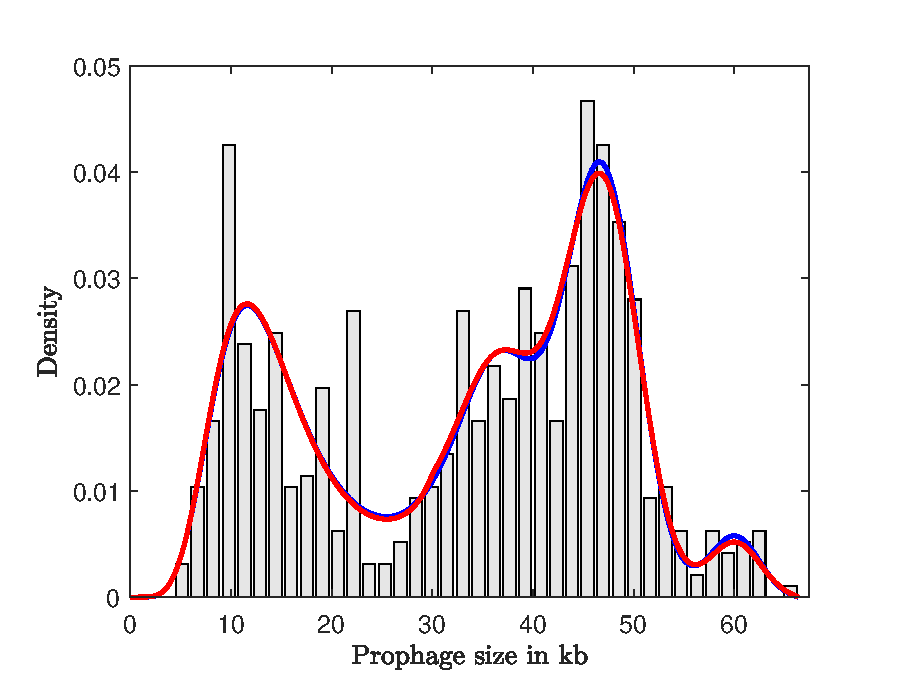
\includegraphics[scale=0.7]{comp_PDF.eps}
\caption[Results of data fitting are not sensitive to the choice of the parameter $\theta$ representing the genome size of the smallest autonomous temperate phage in kb.]{Results of data fitting are not sensitive to the choice of the parameter $\theta$ representing the genome size of the smallest autonomous temperate phage in kb.  Best fits obtained to Data Set 1 (histogram) for $\theta$ = 20 (blue, solid) and $\theta$ = 30 (red, solid) are indistinguishable.}
\label{fig:comp_PDF}
\end{figure}

\subsection{Rate parameters}

We performed a bootstrap sensitivity analysis for all parameters of the model using Data Set 1.  In brief, we assumed that the best fit model for Data Set 1 represented the true distribution, and resampled this true distribution 335 times, each time creating a simulated data set of 624 observed prophage lengths.  We then subjected each of these data sets to the model fitting exercise described in Section 3 of the main text.  Table \ref{table:sens_p} shows the mean and standard deviations for the relative rate parameters of the model (each rate normalized by the induction rate, $r_I$), after the analysis of 335 simulated data sets.  These results indicate that the quantitative conclusions of our work are relatively insensitive to variations in data sampling; the coefficient of variation (standard deviation/mean) of the degradation rate is largest at 16\%.

\renewcommand{\baselinestretch}{1}
\begin{center}
\begin{table}[H]
\centering
\begin{tabular}{ p{1.6cm}p{5cm}p{2cm}p{2cm}p{2.1cm} }
\hline
Parameter & Description  & Mean & Standard deviation & Coefficient of Variation  \\
\hline 
\\
 $\alpha $   & Relative rate of lysogeny &     0.2078&          0.0118 & 0.0569\\
 $r_D$   & Relative rate of degradation &       0.0125&         0.0021 & 0.1644\\
 $r_S$ &   Relative selection coefficient &    0.5012&     0.0483 & 0.0964\\
% $r_I$ & Relative rate of induction & 1.0000 &  ---& --- \\
% \\
 \hline
\end{tabular}
\caption{Sensitivity analysis of rate parameters. }
\label{table:sens_p}
\end{table}
\end{center}

\renewcommand{\baselinestretch}{1.0}

\subsection [Influx of active phage]{Influx of active phage, $f(x)$}

In addition, this process produced 335 estimates of the influx distribution $f(x)$.  In Figure \ref{fig:sens_f}, we plot the mean of these functions at every value of $x$ (blue line), plus/minus one standard deviation (grey area).  The best fit $f(x)$ from Data Set 1 is also shown for comparison (red line).  These results indicate that the form of $f(x)$ is very tightly constrained by the data, a result that is perhaps not surprising given the large number of data points.

\begin{figure}[H]\centering
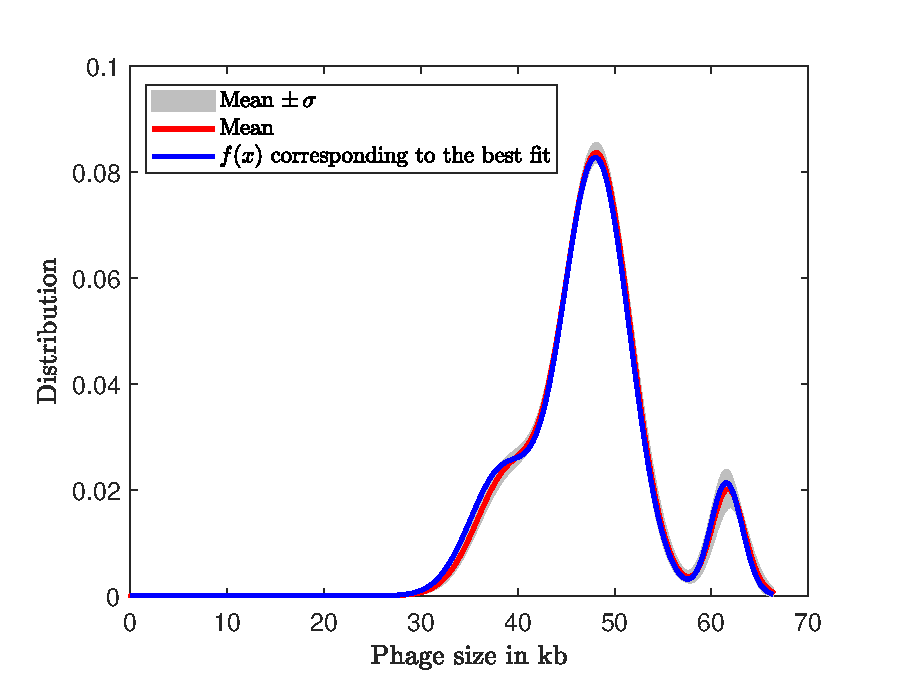
\includegraphics[scale=0.7]{f_sens.eps}

\caption[Sensitivity analysis of the prophage influx function.]{Sensitivity analysis of the prophage influx function.  The mean (red) and standard deviation ($\sigma$) of best-fit $f(x)$ curves for all simulated data sets are shown, along with the best-fit $f(x)$ function from the true data (blue).  See text for details.}
\label{fig:sens_f}
\end{figure}
\addcontentsline{toc}{chapter}{Bibliography}
\bibliographystyle{apa}
\bibliography{refrence}